\chapter{Análise de Requisitos}

\section{Modelo Conceitual}

\begin{figure}[!h]
 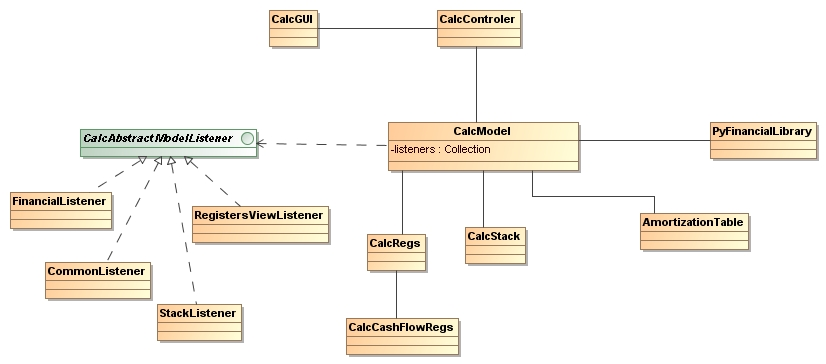
\includegraphics[height = 8cm]{CalcDC.jpg}
 \caption{\it Modelo Conceitual da PyFinancial.} \label{fig:modConc}
\end{figure}

A \ref{fig:modConc} apresenta o modelo conceitual da calculadora financeira, objetivo central desse projeto. É possível identificar algumas entidades centrais desse sistema são elas:

\begin{itemize}
	\item Model
	\item GUI
	\item Controler
	\item AbstractModelListener
	\item Reg
	\item FinancialLibrary
\end{itemize}

\subsection{Model}
Módulo central da aplicação que será responsável por fazer a troca de mensagens entre as demais entidades do sistema as quais está conectada. Também é de sua responsabilidade receber e preparar os dados da aplicação, sejam de entrada ou de saída, formatando-os da forma cujo componente destino requer. Por fim, esta entidade será capaz de tratar a manipulação dos dados da aplicação nos registradores adequados, bem como persistí-los quando necessário.
\subsection{GUI}
Esta é a entidade que estará em contato direto com o usuário da aplicação. Logo, este é o módulo que receberá os dados externos e os transmitirá para entidades mais internas, assim como receberá os resultados das operações realizadas pela calculadora e os transmitirá ao cliente de uma maneira mais amigável.
\subsection{Controler}
Esta entidade é o controlador do sistema. Receberá as requisições feitas pelo cliente da aplicação, através da interface (CalcGUI), e identificará as operações correspondentes na CalcModel que se responsabilizarão por realizar as atividades correspondentes.
\subsection{AbstractModelListener}
Entidade abstrata da qual outras a generalizarão. Estas serão responsáveis por capturar qualquer mudança importante que deva ser refletida na interface, ou seja, mudanças que devão ser mostradas ao usuário.
\subsection{Reg}
Entidade que representa o papel de um registrador. Um registrador é um importante elemento usando para a realização das atividades objetivo da calculadora. Esta entidade será especializada por outras adicionando as particularidades pertinentes aos diverentes tipos de registradores.
\subsection{FinancialLibrary}
Entidade que representa a biblioteca das funções financeiras. Todo e qualquer cálculo financeiro deve chamar a operação correspondente na biblioteca garantindo uma melhor organização e consequentemente, a separação de interesses.


\section{Requisitos}

Durante as reuniões de planejamento entre, os membros da equipe, o cliente e possíveis usuários dos nossos produtos um conjunto de requisitos, funcionais e não funcionais ficaram estabelecidos, são eles:
\begin{itemize}
 \item \textbf{Requisitos Funcionais}
	\begin{itemize}
 	\item O usuário deverá ser capaz de realizar as operações matemáticas seguindo a Notação Polonesa Reversa \cite{NPR}.
	\item O usuário deverá ser capaz de realizar os principais cálculos financeiros (n, i, PV, PMT, FV).
	\item A rolagem automática de valores nos registradores, presentes na HP-12C, deve ser implementada.
	\item Ao finalizar o uso os dados da tela e dos registradores devem ser armazenados em algum tipo de persistência.
	\item A tabela de amortização deve ser mostrada visualmente ao usuário.
	\end{itemize}
 \item \textbf{Requisitos Não-Funcionais}
	\begin{itemize}
	 \item \textbf{Interface}. Possuir interface similar a da calculadora HP12-C, com melhoramentos que possam facilitar sua utilização.
	 \item \textbf{Usabilidade}. O nível de dificuldade encontrado para uso de nossa calculadora deve ser o mesmo encontrado quando faz-se uso das calculadoras tradicionais.
	 \item \textbf{Volume de Utilização}. A calculadora será mono-usuário, porém devendo ser robusta o suficiente para ser utilizada durante um longo intervalo de tempo ininterruptamente sem apresentar problemas.
	 \item \textbf{Hardware e software alvo}. A calculadora deverá funcionar no Internet Tablet N800 da Nokia, no sistema operacional Maemo Diablo (4.1.x) 
	 \item \textbf{Qualidade}. Com relação a precisão, deseja-se que os valores calculados em nossa calculadora não devam diferir em mais de 0.001 unidades dos valores calculados na HP12-C original.
	 \item \textbf{Expressividade nas mensagens}. Entradas equivocadas do usuário deverão apresentar mensagens de erros que sejam mais intuitivas do que as apresentadas pela calculadora original (e.g. "Erro 6").
	 \item \textbf{Desempenho}. O tempo de resposta dos resultados não deve ultrapassar o tempo que a calculadora HP12-C leva para executar as mesmas operações (considerando que só o programa da calculadora esteja em execução).
	 \item \textbf{Segurança}. Os arquivos que conterão os valores dos registradores recém utilizados pelo usuário deverão ficar protegidos de alteração externa.
	 \item \textbf{Compatibilidade}. É desejável que a aplicação possa ser portada para versões mais novas do dispositivo alvo, como o N810, bem como para novas versões do Maemo.
	 \item \textbf{Internacionalização}. A calculadora deve ser desenvolvida para tornar possível a internacionalização. 
	 \item \textbf{Packaging}. A distribuição do aplicativo deve ser realizada através de um arquivo .deb que servirá como instalador para o mesmo.
	\end{itemize}
\end{itemize}
